\documentclass[12pt,a4paper,titlepage]{article}
% Daniel Wong September 10, 2020

\usepackage[fleqn]{amsmath} % To write aligned equations
\usepackage{amssymb} % To write math symbols
\usepackage{graphicx,float} % To add pictures
\usepackage{caption} % To add captions
\usepackage{subcaption} % To add subcaptions
\usepackage{multirow} % To add multirow lines in tables
\usepackage{multicol} % To add multicolumn lines in tables
\usepackage{hyperref} % To add hyperlinks
\usepackage[normalem]{ulem} % To underline
\usepackage[backend=bibtex,citestyle=numeric,autocite=plain,sorting=none]{biblatex} % To add references
\usepackage[english]{babel} % To write accented vowels
\usepackage[toc,page]{appendix} % To add table of contents
\usepackage{physics} % To use supported physics notation
\usepackage[none]{hyphenat} % To remove hyphenation
\usepackage{mathtools}  % To use \mathclap which removes white space for subscripts
\usepackage{tensor} % For subscripts to the left

\usepackage{fancyhdr} % To input custom headers
\pagestyle{fancy} % Defines header for all pages other than plain-style pages
\fancyhf{}
\rhead{\nouppercase\leftmark}
\lfoot{Daniel Wong}
\rfoot{\thepage}
\renewcommand{\headrulewidth}{0.4pt} % Defining width of header line
\renewcommand{\footrulewidth}{0.4pt} % Defining width of footer line

\usepackage{tikz} % To input mathematical plots and diagrams
\usetikzlibrary{decorations.pathreplacing,decorations.pathmorphing,decorations.markings} % For curly braces, wavy lines, and arrow markings
\usetikzlibrary{tikzmark} % For adding annotations to equations
\usetikzlibrary{shapes.geometric} % For drawing regular polygons
\usetikzlibrary{shapes.misc} % For drawing crosses
\usetikzlibrary{snakes} % For drawing zigzag lines
\usetikzlibrary{arrows.meta} % For changing arrow head sizes

\tikzset{->-/.style={decoration={markings,mark=at position #1 with {\arrow{>}}},postaction={decorate}}} 
\tikzset{-<-/.style={decoration={markings,mark=at position #1 with {\arrow{<}}},postaction={decorate}}} % Defining lines with arrows in the middle
\tikzset{cross/.style={cross out,draw,minimum size=2*(#1-\pgflinewidth),inner sep=0pt,outer sep=0pt}} % Defining cross for a node

\usepackage{color} % To use different colours
\usepackage[makeroom]{cancel} % To cancel terms in equations

\definecolor{lightGray}{gray}{0.8}

\newcommand{\trm}[1]{\textrm{#1}} % Shorthand for \textrm command
\newcommand{\up}{\uparrow} % Shorthand for \uparrow command
\newcommand{\dn}{\downarrow} % Shorthand for \downarrow command
\newcommand{\en}{\epsilon_{0}} % Shorthand for \epsilon_{0}
\newcommand{\ul}[1]{\underline{\smash{#1}}} % Properly underlines words
\newcommand{\explain}[1]{% Adds an arrow to allow for explanations in equations
	\quad\rotatebox[origin=c]{180}{\enskip$\Lsh$}\hfill
	\begin{minipage}[t]{\dimexpr\linewidth-8em\relax}
	#1
	\end{minipage}\hspace{4em}\bigskip
}

\newcommand{\aside}[1]{% Aligns the environment for asides
	\ul{Aside}:\hfill
	\begin{minipage}[t]{\dimexpr\linewidth-8em\relax}
	#1
	\end{minipage}\hspace{4em}\bigskip
}

\newcommand{\theorem}[1]{% Aligns the environment for theorems
	\ul{Theorem}:\hfill
	\begin{minipage}[t]{\dimexpr\linewidth-8em\relax}
	#1
	\end{minipage}\hspace{4em}\bigskip
}

\newcommand{\proof}[1]{% Aligns the environment for proof
	\ul{Proof}:\hfill
	\begin{minipage}[t]{\dimexpr\linewidth-8em\relax}
	#1
	\end{minipage}\hspace{4em}\bigskip
}

\newcommand{\definition}[1]{% Aligns the environment for definitions
	\ul{Definition}:\hfill
	\begin{minipage}[t]{\dimexpr\linewidth-8em\relax}
	#1
	\end{minipage}\hspace{4em}\bigskip
}
\newcommand{\example}[2]{% Aligns the environment for examples
	\bigskip
	\hrule
	\bigskip
	\ul{Ex #1}:\hfill
	\begin{minipage}[t]{\dimexpr\linewidth-8em\relax}
	#2
	\end{minipage}\hspace{4em}
	\bigskip
	\hrule
	\bigskip
}

\newcommand{\angstrom}{\textup{\AA}} % Angstrom symbol
\newcommand{\Chi}{\mathcal{X}} % Inline chi symbol
\newcommand{\Tau}{\mathcal{T}} % Capital tau symbol
\newcommand{\sign}{\trm{sign}} % Sign function
\newcommand{\pd}[1]{\partial_{#1}} % Covariant 4-gradient
\newcommand{\pu}[1]{\partial^{#1}} % Contravariant 4-gradient
\newcommand{\id}{\mathbb{I}} % Identity matrix
\renewcommand{\Re}{\trm{Re}} % Real
\renewcommand{\Im}{\trm{Im}} % Imaginary
\renewcommand{\CancelColor}{\color{red}} % Changes the cancel colour to red

\begin{document}
\title{ELEC 542: Nanoscale Modelling}
\author{Daniel Wong\\University of British Columbia\\Instructor: Dr. Alireza Nojeh}
\date{Winter 2022}
\maketitle

\setlength\parindent{0pt}
\pagenumbering{roman}
\numberwithin{equation}{section}

\section*{Disclaimer}
These notes may be freely used by anyone who comes across them. If any errors are found within these notes, please email me at \ul{temp@temp.com}. If you are the previous instructor of this course (Dr. Alireza Nojeh) and have concerns about keeping these notes on my website, please contact me at the email provided.\\

Other course notes may be found on my website at \url{www.temp.com/notes}.

\newpage
\tableofcontents
\newpage
\pagenumbering{arabic}

\section{Introduction}
Note the challenge of simulating systems at the nanoscale: too many particles to keep track of but not enough particles to treat statistically and as a continuum.\\

In the context of this course, the equation of motion for electrons is the Schr\"{o}dinger equation and the nucleus will be considered as point particles.\\

The map of the course content is as follows:
\begin{center}
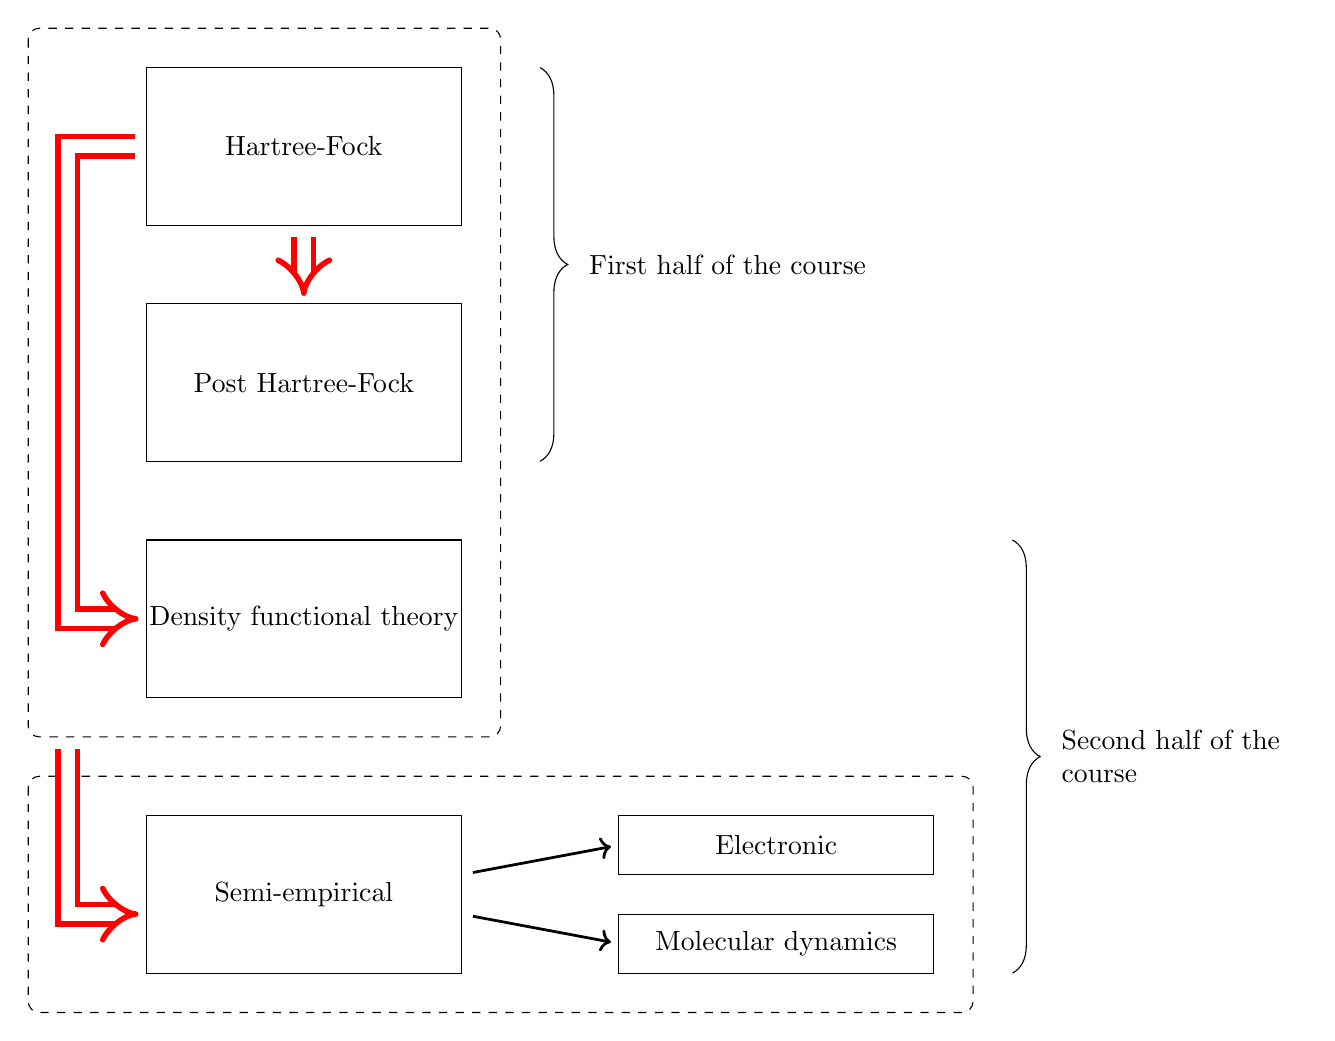
\begin{tikzpicture}
	\draw (0,0) rectangle node{Hartree-Fock} (4,2);
	\draw[red,-{Implies},shorten >=1mm,shorten <=1.5mm,double distance=5pt,line width=2 pt] (2,0) -- (2,-1);
	\draw (0,-1) rectangle node[align=center,text width=4cm]{Post Hartree-Fock} (4,-3);
	\draw (0,-4) rectangle node[align=center,text width=4cm]{Density functional theory} (4,-6);
	\draw[red,-{Implies},shorten >=1mm,shorten <=1.5mm,double distance=5pt,line width=2 pt] (0,1) -- (-1,1) -- (-1,-5) -- (0,-5);
	\draw[dashed,rounded corners] (-1.5,2.5) rectangle (4.5,-6.5);
	\draw (0,-7.5) rectangle node[align=center,text width=4cm]{Semi-empirical} (4,-9.5);
	\draw (6,-7.5) rectangle node[align=center]{Electronic} (10,-8.25);
	\draw (6,-8.75) rectangle node[align=center]{Molecular dynamics} (10,-9.5);
	\draw[dashed,rounded corners] (-1.5,-7) rectangle (10.5,-10);
	\draw[red,-{Implies},shorten >=1mm,shorten <=1.5mm,double distance=5pt,line width=2 pt] (-1,-6.5) -- (-1,-8.75) -- (0,-8.75);
	\draw[->,shorten >=1mm,shorten <=1.5mm,line width=1 pt] (4,-8.25) -- (6,-7.875);
	\draw[->,shorten >=1mm,shorten <=1.5mm,line width=1 pt] (4,-8.75) -- (6,-9.125);
	\draw[decorate,decoration={brace,amplitude=10pt}] (5,2) -- (5,-3) node[right,midway,xshift=0.5cm] {First half of the course};
	\draw[decorate,decoration={brace,amplitude=10pt}] (11,-4) -- (11,-9.5) node[right,midway,xshift=0.5cm,text width=3cm] {Second half of the course};
\end{tikzpicture}
\end{center}

Let us consider the Schr\"{o}dinger equation for a system.
\begin{equation}
	\tikzmarknode{A}{\vb{H}}\tikzmarknode{B}{\Psi}=\tikzmarknode{C}{E}\Psi \quad (\trm{time-independent})
\end{equation}
\begin{tikzpicture}[overlay,remember picture,shorten <=1mm,font=\footnotesize]
	\draw[red,<-] (A.south) -- ++ (-0.3,-0.3) node[left,xshift=0.1cm,yshift=-0.1cm] {Hamiltonian};
	\draw[red,<-] (B.south) -- ++ (0,-0.5) node[below] {wavefunction};
	\draw[red,<-] (C.south) -- ++ (0.3,-0.3) node[right,xshift=-0.1cm,yshift=-0.1cm] {energy eigenvalue};
\end{tikzpicture}

The wavefunction is a function of all the electron and nuclei coordinates
\begin{equation}
	\Psi=\Psi\qty(\vec{r}_{1},\ldots,\vec{r}_{N},\vec{R}_{1},\ldots,\vec{R}_{M})\quad(\trm{many-body wavefunction})
\end{equation}

\begin{center}
\begin{tikzpicture}
	\draw[ultra thick,->] (0,0) -- (0,4) node[above]{$z$};
	\draw[ultra thick,->] (0,0) -- (4,0) node[right]{$y$};
	\draw[ultra thick,->] (0,0) -- (-1,-1) node[below left]{$x$};
	\draw[->] (0,0) -- (1,2) node[above]{$\vec{r}_{i}$};
	\draw[->] (0,0) -- (3,1.5) node[right]{$\vec{R}_{A}$};
	\node[right] at (5,3) {$i=1,\ldots,N$ (number of e$^{-}$)};
	\node[right] at (5,2) {$A=1,\ldots,M$ (number of nuclei)};
\end{tikzpicture}
\end{center}

The Hamiltonian of the system is as follows
\begin{equation}
\begin{aligned}
\vb{H}&=\color{red}\underbrace{\color{black}\sum_{i=1}^{N}-\frac{1}{2}\nabla_{i}^{2}}_{\trm{e$^{-}$ KE}}\quad{\color{black}+}\quad\underbrace{\color{black}\sum_{A=1}^{M}-\frac{1}{2M_{A}}\nabla_{A}^{2}}_{\trm{nuclei KE}}\quad{\color{black}+}\quad\underbrace{\color{black}\sum_{i=1}^{N}\sum_{j>i}^{N}\frac{1}{r_{ij}}}_{\trm{e$^{-}$-e$^{-}$ repulsion}}\\
&\color{red}\quad{\color{black}+}\quad\underbrace{\color{black}\sum_{A=1}^{M}\sum_{B>A}^{M}\frac{Z_{A}Z_{B}}{R_{AB}}}_{\trm{nucleus-nucleus repulsion}}\quad{\color{black}+}\quad\underbrace{\color{black}\sum_{i=1}^{N}\sum_{A=1}^{M}-\frac{Z_{A}}{r_{iA}}}_{\trm{e$^{-}$-nucleus repulsion}}
\end{aligned}
\end{equation}

This is the (non-relativistic) theory of everything. Note that this is written in atomic coordinates (hence the mass and charge of electrons are 1). Note that spin is also missing from the equation above.\\

In condensed matter physics, one gets accustomed to imagining quasi-particles. These quasi-particles are models of a higher-abstraction that helps give insight into the behaviour of the system. Rather than appearing to neglect this quasi-particle picture in the Hamiltonian above, the picture comes out from the Hamiltonian equation. At the start of this course, we will want to solve this Hamiltonian without jumping straight away to the usage of quasi-particles or using approximations.\\

Let us also make a note about states. Consider a carbon atom.
\begin{center}
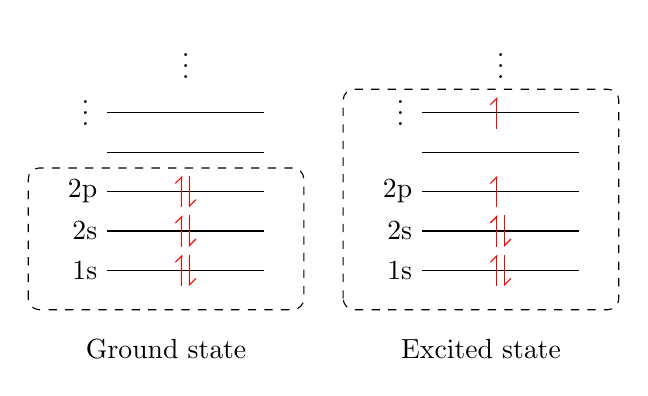
\begin{tikzpicture}
	\draw (0,0) node[left] {1s} -- (2,0);
	\draw [red,-{Straight Barb[left]}] (0.95,-0.2) -- (0.95,0.2);
	\draw [red,-{Straight Barb[left]}] (1.05,0.2) -- (1.05,-0.2);
	\draw (0,0.5) node[left] {2s} -- (2,0.5);
	\draw [red,-{Straight Barb[left]}] (0.95,0.3) -- (0.95,0.7);
	\draw [red,-{Straight Barb[left]}] (1.05,0.7) -- (1.05,0.3);
	\draw (0,1) node[left] {2p} -- (2,1);
	\draw [red,-{Straight Barb[left]}] (0.95,0.8) -- (0.95,1.2);
	\draw [red,-{Straight Barb[left]}] (1.05,1.2) -- (1.05,0.8);
	\draw (0,1.5) -- (2,1.5);
	\draw (0,2) node[left,yshift=0.1cm,xshift=-0.1cm] {$\vdots$} -- (2,2);
	\node at (1,2.7) {$\vdots$};
	\draw[dashed,rounded corners] (-1,-0.5) rectangle (2.5,1.3);
	\draw (4,0) node[left] {1s} -- (6,0);
	\draw [red,-{Straight Barb[left]}] (4.95,-0.2) -- (4.95,0.2);
	\draw [red,-{Straight Barb[left]}] (5.05,0.2) -- (5.05,-0.2);
	\draw (4,0.5) node[left] {2s} -- (6,0.5);
	\draw [red,-{Straight Barb[left]}] (4.95,0.3) -- (4.95,0.7);
	\draw [red,-{Straight Barb[left]}] (5.05,0.7) -- (5.05,0.3);
	\draw (4,1) node[left] {2p} -- (6,1);
	\draw [red,-{Straight Barb[left]}] (4.95,0.8) -- (4.95,1.2);
	\draw [red,-{Straight Barb[left]}] (4.95,1.8) -- (4.95,2.2);
	\draw (4,1.5) -- (6,1.5);
	\draw (4,2) node[left,yshift=0.1cm,xshift=-0.1cm] {$\vdots$} -- (6,2);
	\node at (5,2.7) {$\vdots$};
	\draw[dashed,rounded corners] (3,-0.5) rectangle (6.5,2.3);
	\node at (0.75,-1) {Ground state};
	\node at (4.75,-1) {Excited state};
\end{tikzpicture}
\end{center}
Note that the entire population of electrons in this configuration is the ground state. In a one-electron picture, one may grow accustomed to thinking of the 1s orbital as the ground state, which we will want to move away from.

\section{Hartree-Fock}
Let us try to decouple this problem into two problems: an electronic portion and a nuclei portion.

\subsection{Born-Oppenheimer Approximation}
Note that the mass of the nucleus is many orders of magnitude larger than the mass of the electron. One should expect that the nuclei moves much slower than the electrons.\\

One can make the Born-Oppenheimer approximation. At a given moment in time, we assume that the nuclei are fixed and that the electrons are moving in the background of these fixed nuclei.\\

Thus, the variables $\vec{R}_{1},\ldots,\vec{R}_{M}$ now represent fixed positions. The second term of the Hamiltonian now drops out and the fourth term just becomes a fixed constant. We now treat the many-body wavefunction as
\begin{equation}
\Psi=\Psi_{\trm{elec}}(\color{red}\underbrace{\color{black}\vec{r}_{1},\ldots,\vec{r}_{N}}_{\substack{\trm{explicit}\\\trm{variables}}},\underbrace{\color{black}\vec{R}_{1},\ldots,\vec{R}_{M}}_{\trm{parameters}}{\color{black})\Psi_{\trm{nucl}}(}\underbrace{\color{black}\vec{R}_{1},\ldots,\vec{R}_{M}}_{\substack{\trm{explicit}\\\trm{variables}}}{\color{black})}
\end{equation}
The methodology for solving the motion of the system thus starts with solving the many-body electronic problem in the background of fixed nuclei. From this solution, one can calculate the forces acting on the nuclei from the electronic cloud and other nuclei and evolve the nuclei by one time-step. One then again makes the Born-Oppenheimer approximation and recalculates the electronic solution in the new background of fixed nuclei. These steps are then iterated to find the motion of the system in a ``quasi-static" manner.\\

Note for the nuclei portion, one is not looking at the effects of fixed electrons in space acting on the nuclei. Rather one is looking at the average effects by the electron cloud on the nuclei. Thus, $\Psi_{\trm{nucl}}$ does not parametrically depend on the electron coordinates.\\

Thus, in more detail
\begin{equation}
\begin{aligned}
\vb{H}\Psi&=\qty(\sum_{i=1}^{N}-\frac{1}{2}\nabla_{i}^{2}\Psi_{\trm{elec}})\Psi_{\trm{nucl}}+\qty(\sum_{A=1}^{M}-\frac{1}{2M_{A}}\nabla_{A}^{2}\qty(\Psi_{\trm{elec}}\Psi_{\trm{nucl}}))\\
&\quad+\qty(\sum_{i=1}^{N}\sum_{j>i}^{N}\frac{1}{r_{ij}})\Psi_{\trm{elec}}\Psi_{\trm{nucl}}+\qty(\sum_{A=1}^{M}\sum_{B>A}^{M}\frac{Z_{A}Z_{B}}{R_{AB}})\Psi_{\trm{elec}}\Psi_{\trm{nucl}}\\
&\quad+\qty(\sum_{i=1}^{N}\sum_{A=1}^{M}-\frac{Z_{A}}{r_{iA}})\Psi_{\trm{elec}}\Psi_{\trm{nucl}}
\end{aligned}
\end{equation}

\end{document}